\documentclass{amsart}

%%%%%%%%%%%%%%%

\usepackage[utf8]{inputenc}
% \usepackage[spanish]{babel}
% \usepackage[top=1in, bottom=1in, left=1.2in, right=1.2in]{geometry}
\usepackage{amssymb}
\usepackage{amsmath}
\usepackage{amsfonts}
\usepackage{amsthm}
\usepackage{wasysym}
\usepackage{enumitem}
\usepackage{graphicx}
\usepackage{listings}
\usepackage{xcolor}
\usepackage{tikz}

% sets
\newcommand{\NN}{\mathbf{N}}
\newcommand{\ZZ}{\mathbf{Z}}
\newcommand{\QQ}{\mathbf{Q}}
\newcommand{\RR}{\mathbf{R}}
\newcommand{\Zpos}{\ZZ^{+}}
\newcommand{\Rpos}{\RR^{+}}

% brackets
\newcommand{\la}{\langle}
\newcommand{\ra}{\rangle}

% formal statements
\newtheorem{prop}{Proposition}

\theoremstyle{plain}
\newtheorem{clm}{Claim}

\theoremstyle{definition}
\newtheorem{defn}{Definition}

\newtheorem{exl}{Example}

\theoremstyle{remark}
\newtheorem{rmk}{Remark}

% vulgar display of code

\lstdefinestyle{astyle}{
	commentstyle=\color{blue},
	keywordstyle=\color{purple},
	numberstyle=\tiny\color{gray},
	stringstyle=\color{green},
	basicstyle=\ttfamily\footnotesize,
	tabsize=2
}

\lstset{style=astyle}


\title{Work log of June 13 2025}
\author{Daniel R. Barrero R.}
% \date{\today}

\begin{document}

\maketitle

\section{General}

\begin{itemize}
	\item In \texttt{splitForest}, the typed value \texttt{(lrdr,krdr)} is
		matched against the typed value \texttt{plusAssoc j1 j2' j2''}.
	\item All relevant \emph{code} written. Now dealing with compilation
		errors, mainly \emph{coercion} for cases of type-level 
		addition.
	\item \texttt{Proxy} is a polymorphic singleton type.
\end{itemize}

\newpage

\section{Type signatures and function evaluations}

\bigskip
\bigskip

\subsection{}

The type signature of the \texttt{splitForest} function is

\lstinputlisting[language=Haskell, firstline=17, lastline=22]{DocCode.hs}

\bigskip
\bigskip

And the evaluation of its recursive case is given by

\lstinputlisting[language=Haskell, firstline=23, lastline=34]{DocCode.hs}

\bigskip
\bigskip

this can be visualized in the following picture:

\bigskip
\bigskip

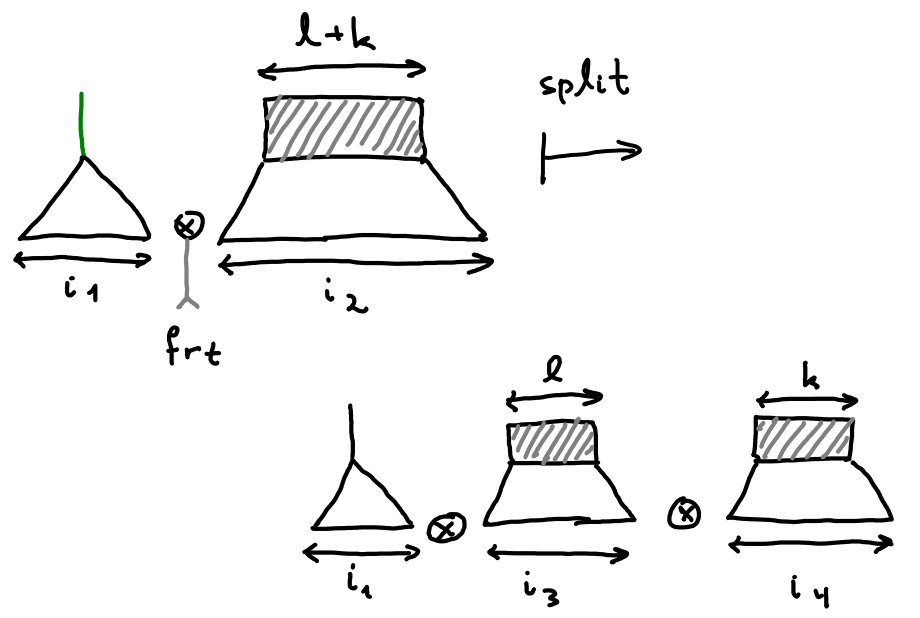
\includegraphics[width=0.8\textwidth]{forestSplit.png}

\newpage

\subsection{} 

The signature of the \texttt{Operad} typeclass is

\lstinputlisting[language=Haskell, firstline=9, lastline=11]{DocCode.hs}

\bigskip
\bigskip

And our instance of interest is the type \texttt{MoveTree}, which is
parametrized by the \texttt{Nat} kind. Its signature is coupled with
that of \texttt{Trees}, also parametrized by \texttt{Nat}. These signatures
are

\lstinputlisting[language=Haskell, firstline=1, lastline=7]{DocCode.hs}

\bigskip
\bigskip

Therefore, the main challenge in making move trees an operad instance is
defining the \texttt{compose} function, especially in the recursive case.

\bigskip

Here's an overview of the instantiation:

\lstinputlisting[language=Haskell, firstline=36, lastline=46]{DocCode.hs}

This depicts the composition arguments:

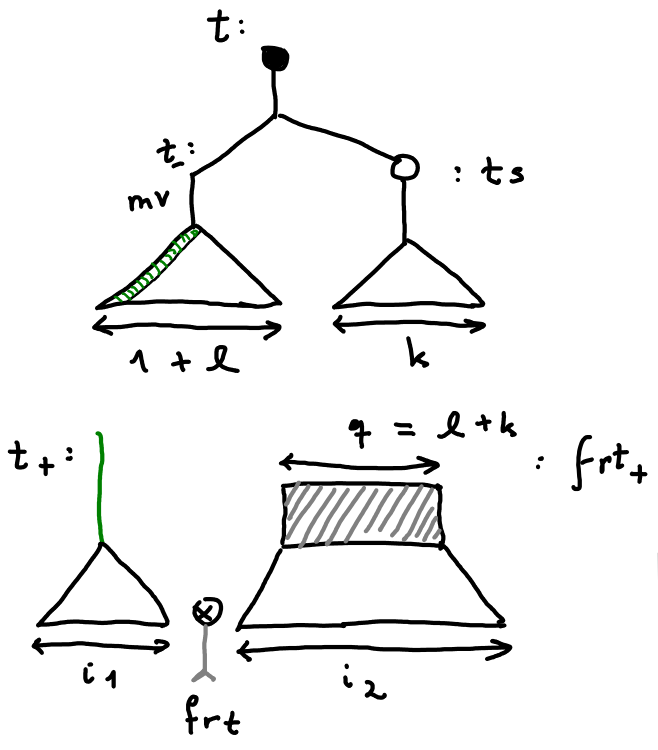
\includegraphics[width=0.7\textwidth]{bigPic.png}

And this is a scheme of the composition's result:

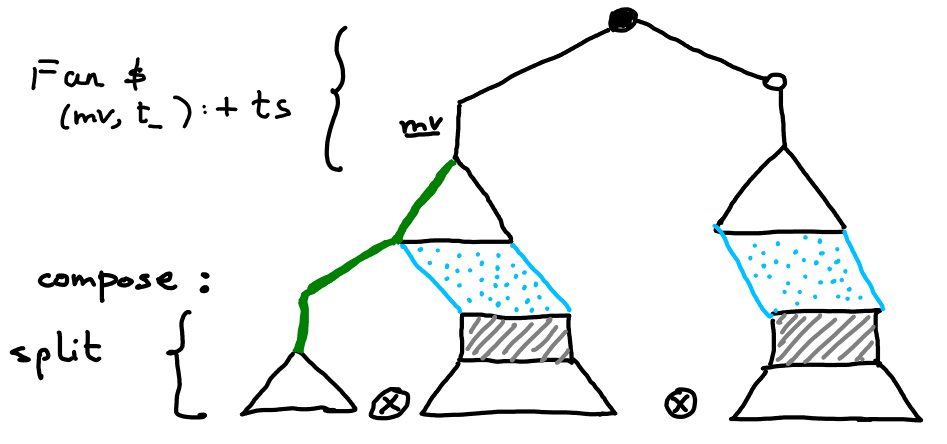
\includegraphics[width=0.7\textwidth]{result.png}

\end{document}
